\documentclass{beamer}
\usepackage[utf8]{inputenc}
\usetheme{Copenhagen}
%\usetheme{CambridgeUS}

\usepackage[export]{adjustbox}

\title{Personality Traits Analysis from Forum Dataset}
\author{Angeliki Theodorou, Lirije Tahiri, Frederike Gartzky}
%\institute{Overleaf}
%\date{2014}

\begin{document}
	\frame{\titlepage}
	
	\begin{frame}
		\frametitle{Project tasks}
		\begin{enumerate}
			\item Extract text from reddit using BeautifulSoup.% filtered by subreddit and keyword or subreddit and username.
			\item Identify text related to each user and select users according to some properties.
			\item Install and run the big-five personality trait implementation in \href{url}{https://github.com/SenticNet/personality-detection} with sample text.
			%\item Test and discuss the analysis using a social media dataset of our choice (in our case reddit).
			\item Link the output of the webcrawler with the personality trait classification and implement a program that gets a single user as input and outputs their personality trait.
			\item Compute semantic similarity of messages and predefined keywords associated with the personality traits.
			\item Create a GUI, enabling the user to filter by subreddit and keyword or subreddit and username.
		\end{enumerate}
	\end{frame}
	
	\begin{frame}
		\frametitle{Background: 5 personality traits}
		\begin{tabular}{cl}
			\begin{tabular}{c}
				\parbox{0.35\linewidth}{
					OCEAN:
				\begin{itemize}
					\item Openness
					\item Conscientiousness
					\item Extroversion
					\item Agreeableness
					\item Neuroticism
				\end{itemize}
				} 
			\end{tabular}
			\begin{tabular}{l}
				\parbox{0.65\linewidth}{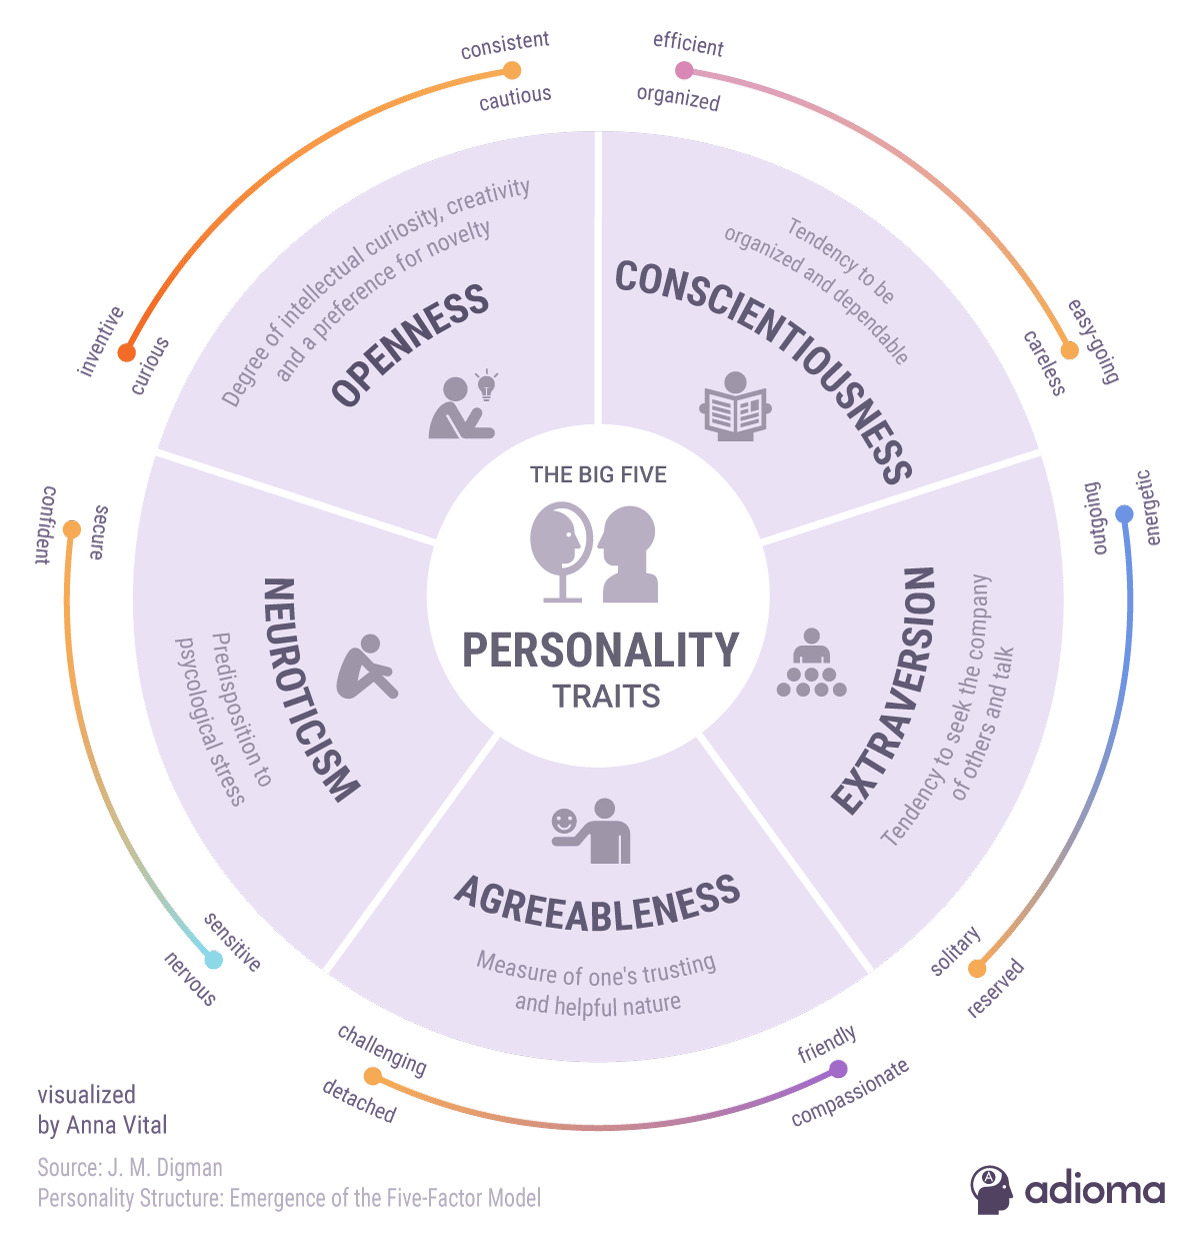
\includegraphics[height=.7\textheight]{pictures/traits2.jpeg}}
			\end{tabular}
		\end{tabular}
	\end{frame}


\begin{frame}
	\frametitle{What we have done so far}
	\begin{itemize}
		\item GUI using Tkinter
		\item extraction of text from reddit using BeautifulSoup
		\item used library multiprocessing for threading
		\item installed and tested personality detection framework
	\end{itemize}
\end{frame}





\begin{frame}
\frametitle{GUI}
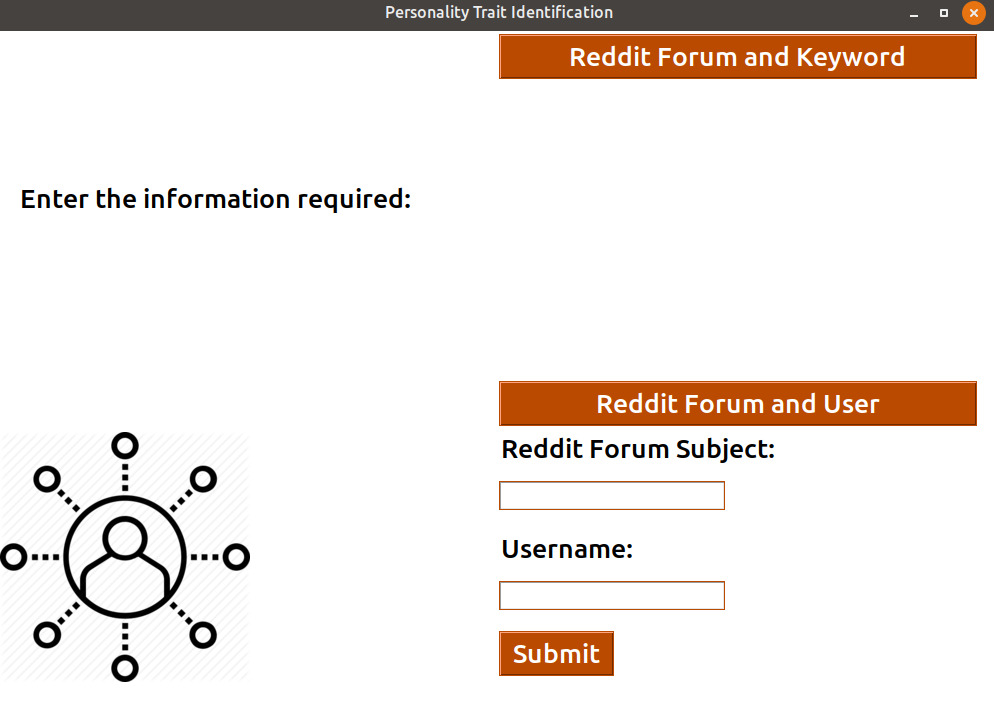
\includegraphics[width=\textwidth]{pictures/gui3}
\end{frame}

\begin{frame}
\frametitle{GUI}
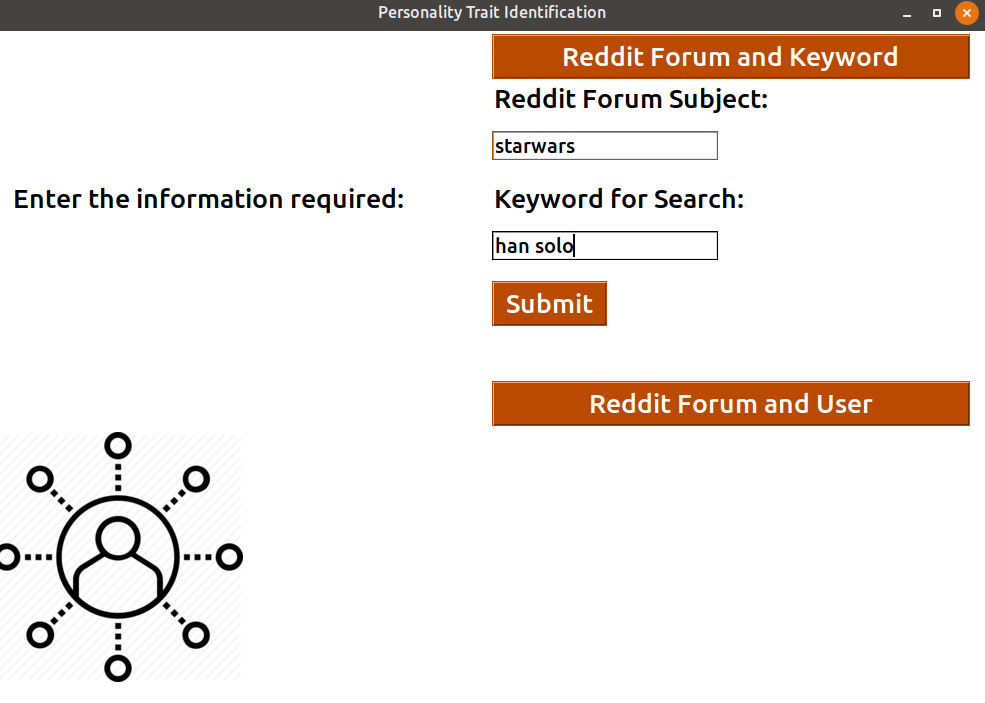
\includegraphics[width=\textwidth]{pictures/gui4}
\end{frame}


	\begin{frame}
		\frametitle{Extracted Text from reddit}
		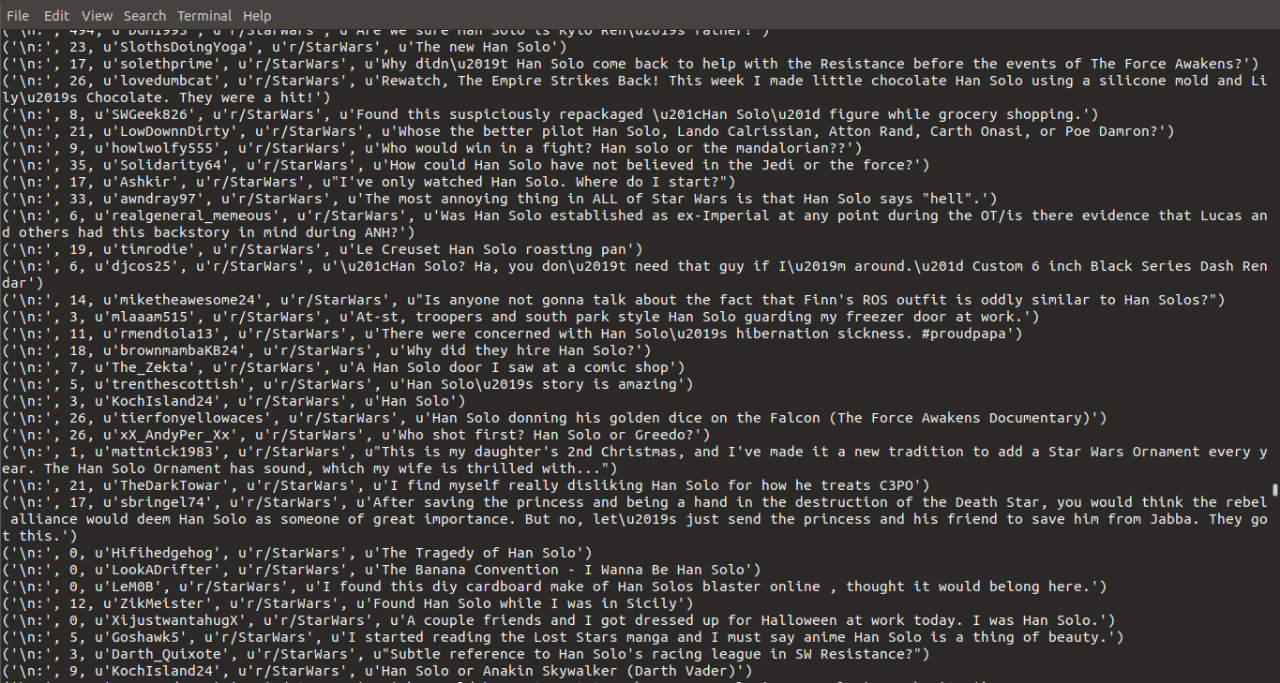
\includegraphics[width=\textwidth]{pictures/crawl1}
	\end{frame}

	\begin{frame}
\frametitle{How does the given framework work?}
Deep Learning-Based Personality Detection\cite{traitpaper}
\begin{itemize}
	\item Preprocessing: sentence splitting, cleaning
	\item Document-level feature extraction: Mairesse baseline feature set
	\item Filtering: ignore sentences that don't carry any personality cues
	\item Word-level feature extraction: word2vec representation 
	\item Classification: deep CNN
\end{itemize}
\end{frame}


	\begin{frame}
		\frametitle{Personality Trait Classification with given Framework}
		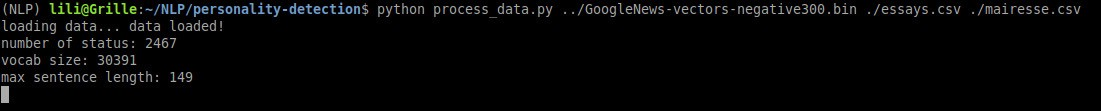
\includegraphics[width=\textwidth]{pictures/output3}
		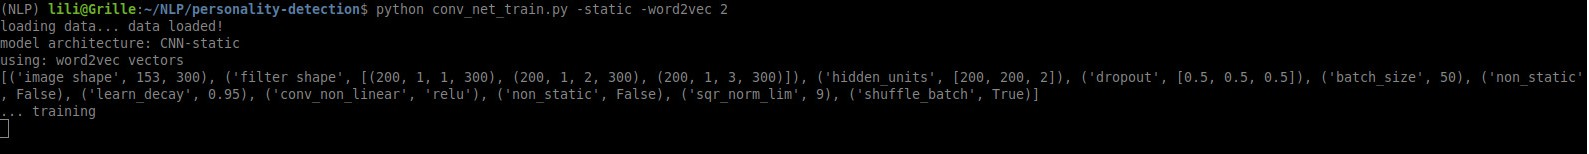
\includegraphics[width=\textwidth]{pictures/output1}		
	\end{frame}

	\begin{frame}
		\frametitle{What next?}
		Todo:
		\begin{itemize}
			\item Link the crawly output with the personality trait classifier.
			\item Program that takes data of a user and outputs the respective personality trait.
			\item Personality trait classifier using keywords and semantic similarity, compare results.
		\end{itemize}
	
		Sharing the work
		\begin{itemize}
			\item divide all tasks evenly
			\item still collaborate and help each other
		\end{itemize}
	\end{frame}

	\begin{frame}
		\frametitle{References}
		\begin{thebibliography}{9}
			\setbeamertemplate{bibliography item}[text]
			\bibitem{traitpaper}
			N. Majumder, S. Poria, A. Gelbukh, E. Cambria,
			\textit{Deep Learning-Based
				Document Modeling
				for Personality
				Detection from Text},
			IEEE Intelligent Systems,
			2017
			\bibitem{traitpic}
			\textit{Personality traits picture}
			\url{https://blog.adioma.com/5-personality-traits-infographic/}
			%\bibitem{edgebundle}
			%Danny Holten,
			%\textit{Hierarchical Edge Bundles: Visualization of Adjacency Relations in Hierarchical Data},
			%IEEE Transactions on Visualization and Computer Graphics, 2006
			%\bibitem{kdpic}
			%S. Chen, D. Laefer, E. Mangina,
			%\textit{State of Technology Review of Civilian UAVs},
			%Recent Patents on Engineering, 2016
			%\bibitem{octreepic}
			%WhiteTimberwolf, \textit{Octree}, \url{https://commons.wikimedia.org/w/index.php?curid=9851485}
			%\bibitem{compgeo}
			%M. de Berg, O. Cheong, M. van Kreveld, M. Overmars,
			%\textit{Computational Geometry},
			%Springer, 2008
		\end{thebibliography}
	\end{frame}
	
\end{document}